% master: l2kurz.tex
% L2K4.TEX - 4.Teil der LaTeX2e-Kurzbeschreibung v2.2
% L2K4.TEX - 4.Teil der LaTeX2e-Kurzbeschreibung Mainz 1994, 1995
% LK4.TEX  - 4.Teil der LaTeX-Kurzbeschreibung Graz-Wien 1987
% last changes: 2001-06-10 (WaS)

\section{Setzen von Bildern} \label{graphics}
Lädt man im Vorspann des Dokuments das Paket \texttt{graphicx},
dann kann man Bilder, die mit einem anderen Programm erzeugt wurden, 
mit dem Befehl \verb|\includegraphics| in das Dokument einfügen.
Der Dateiname ist als Argument des Befehls anzugeben.
Welche Dateiformate verarbeitet werden können, hängt vom jeweiligen
\TeX-System ab und muss in dessen Dokumentation beschrieben sein.

\exa
Hier 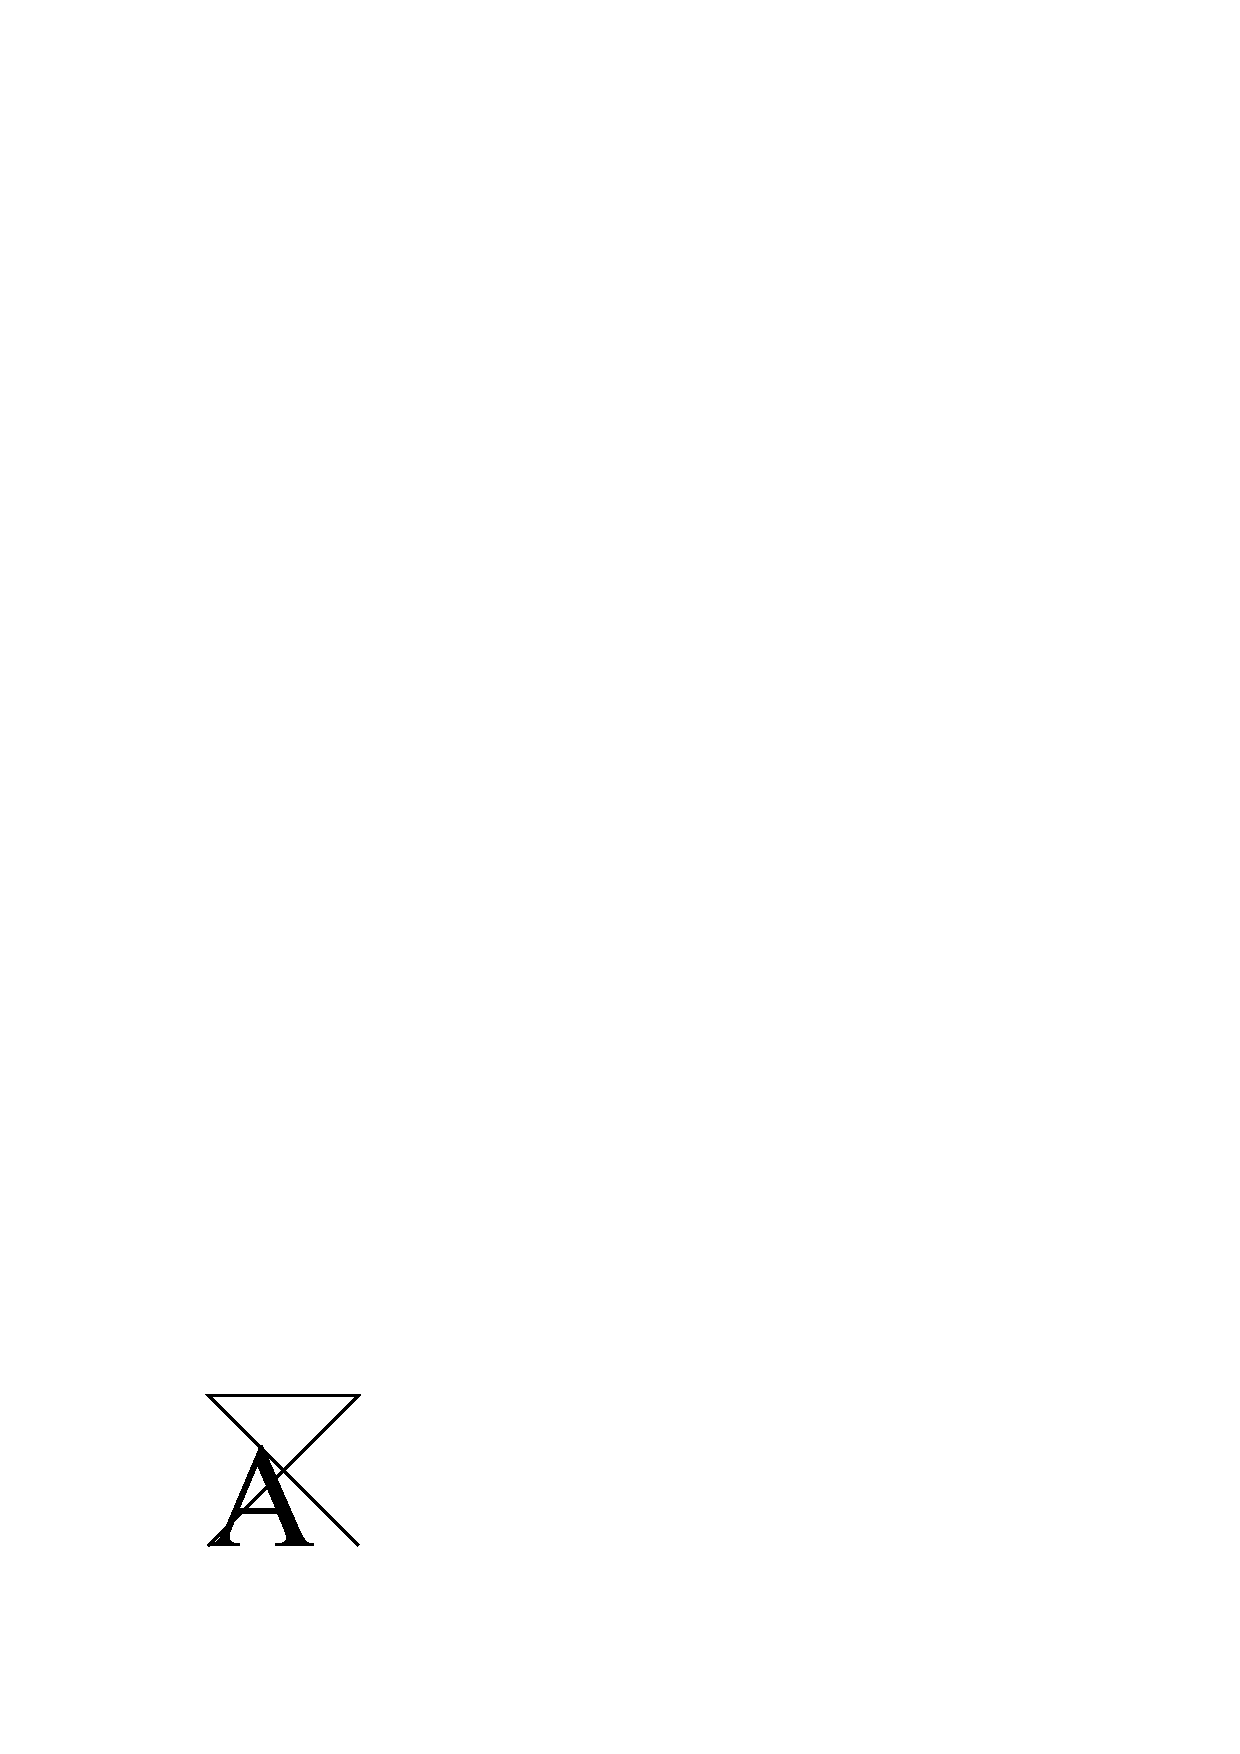
\includegraphics{a} ist ein Bild.
\exb
\begin{verbatim}
Hier 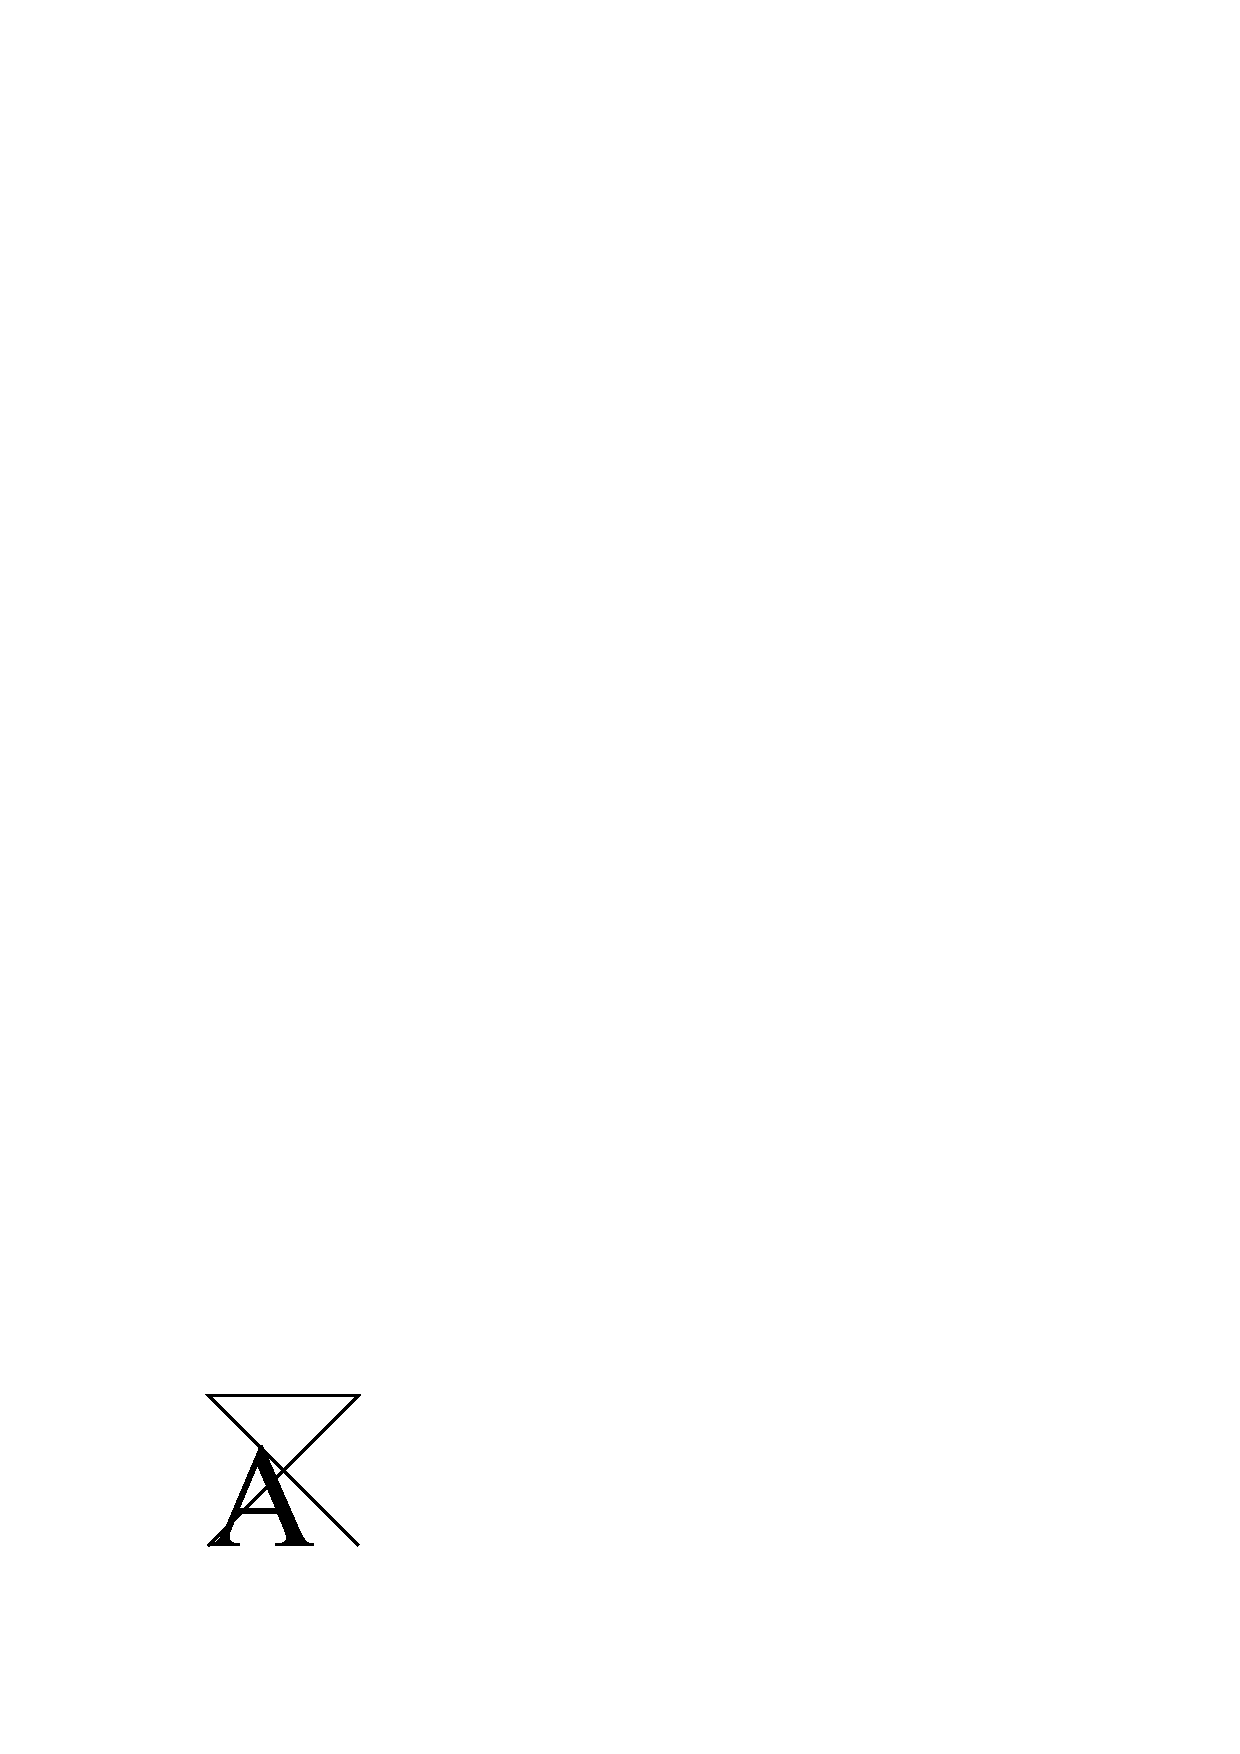
\includegraphics{a} ist
ein Bild
\end{verbatim}
\exc
Wird das Paket \texttt{graphicx} mit der Option \texttt{[draft]} geladen,
dann erscheint anstelle des Bildes nur ein Rahmen entsprechend
der tatsächlichen Bildgröße mit dem Namen des Grafikfiles, 
was die Bearbeitung beschleunigt und für Probeausdrucke nützlich ist.

Weitere Informationen zum Enbinden von Bildern finden Sie in der 
Online-Dokumentation \cite{grfguide}, im \textit{Graphics Companion}
\cite{grfcomp} und in K.~Reckdahls empfehlenswertem  Tutorium \cite{epslatex}.



\section{Seitenaufbau}

\subsection{Kopf- und Fußzeilen} 
Der Inhalt von Kopf- und  Fußzeilen kann mit dem Befehl
\begin{verse}
\verb|\pagestyle{|\textit{style}\verb|}|
\end{verse}
festgelegt werden:
 
Mit \verb|\pagestyle{plain}| steht
die Seitennummer zentriert in der Fußzeile; 
das ist die Voreinstellung und braucht normalerweise nicht explizit 
angegeben zu werden.
Mit dem Stil \texttt{headings} stehen Kapitel-Überschrift und
Seitennummer in der Kopfzeile.
Mit \texttt{empty} sind Kopf- und Fußzeile leer.  Der Befehl
\begin{verse}
\verb|\thispagestyle{|\textit{style}\verb|}|
\end{verse}
gilt entsprechend nur für die aktuelle Seite.  Einige Befehle, wie etwa
\verb|\chapter|, ändern den Stil der aktuellen Seite.  Diese Änderungen 
kann man durch einen nachfolgenden \verb|\thispagestyle|-Befehl aufheben.

\begin{sloppypar}%% `sloppypar'-Umgebung wegen vieler Befehle
\hbadness=4600\relax %% `underfull hbox'-Fehlermeldung aus
Im \manual\ ist angegeben, wie man das Aussehen der Kopf- und Fußzeilen
außerdem mit dem Seitenstil 
\verb|myheadings| und den Befehlen
\verb|\markboth|,
\verb|\markright| und
\verb|\pagenumbering|
beeinflussen kann.
\end{sloppypar}

\subsection{Gleitobjekte} \label{floats}
Große Bilder und lange Tabellen lassen sich nicht immer genau 
dort unterbringen, wo sie inhaltlich hingehören, weil sie nicht mehr 
vollständig auf die aktuelle Seite passen, aber auch nicht durch einen 
Seitenwechsel zerrissen werden sollen.  Um  solche Strukturen automatisch
an eine geeignete Stelle "`gleiten"' zu lassen, kennt \LaTeX{} die beiden 
Umgebungen \texttt{figure} und \texttt{table}.  

\subsubsection{Abbildungen (figure)}
Diese Umgebung ist für die Behandlung von Abbildungen gedacht.
Tatsächlich spielt es aber keine Rolle, \emph{wie} diese erzeugt wurden:
Alles, was zwischen
\verb|\begin{figure}| und \verb|\end{figure}|
steht, wird automatisch an eine Stelle
gesetzt, wo es komplett hinpasst, ohne durch einen Seitenwechsel
zerrissen zu werden.  

Mit \verb|\caption{...}| setzt man die Bezeichnung der Abbildung.
Dabei ist nur der Text anzugeben, das Wort "`Abbildung"' und die
fortlaufende Nummer werden von \LaTeX\ hinzugefügt.
Bei Abbildungen ist es allgemein üblich, die Bezeichnung
\emph{unter} das Bild zu setzen.
Mit \verb|\label| und \verb|\ref| kann man die Nummer der
Abbildung im Text ansprechen, mit \verb|\pageref| ihre Seitenzahl.
Der Befehl \verb:\label: muss dabei \emph{nach} dem \verb:\caption:-Befehl
stehen, sonst stimmt die Numerierung nicht!

Im folgenden Beispiel wird einfach mit dem Befehl \verb|\vspace|
(siehe Abschnitt \ref{vabstaende})
leerer Raum für ein später einzusetzendes Bild gelassen:
\exa
Abbildung~\ref{weiss} auf S.~\pageref{weiss} zeigt ein
Beispiel aus der Minimal art.
\exb
\begin{verbatim}
Abbildung~\ref{weiss} auf
S.~\pageref{weiss} zeigt
ein Beispiel aus der 
Minimal art.
\begin{figure}[tb]
\vspace{6cm}
\caption{Landschaft im
Nebel} \label{weiss}
\end{figure}
\end{verbatim}
\exc
\begin{figure}[tb]
\vspace{6cm}
\caption{Landschaft im
Nebel} \label{weiss}
\end{figure}

\LaTeX\ kann eine Abbildung nach verschiedenen Kriterien plazieren:
\texttt{h} "`here"' (hier),
\texttt{t} "`top"' (oben auf der Seite), \texttt{b} "`bottom"' (unten
auf der Seite) oder \texttt{p} "`page"' (eigene Seite für
Abbildungen).

Die Parameter in den eckigen Klammern, die wahlweise angegeben
werden können, dienen dazu, die Plazierung der Abbildung auf die
angegebenen Orte \emph{einzuschränken}.  Durch Angabe von
z.\,B.\ \texttt{tb}
wird \LaTeX{} angewiesen, nur eine Plazierung oben oder unten auf der
Seite zu versuchen, je nachdem,
wo \emph{zuerst} eine passende Stelle gefunden wird.
Werden keine Parameter (und keine eckigen
Klammern!) angegeben, ist die Voreinstellung \texttt{tbp},
also ohne~\texttt{h}.

Eine Plazierungsbeschränkung \emph{nur} auf \texttt{[h]} ist unsinnig;
sie würde das "`Gleiten"' ja gerade verhindern.
Wenn der Platz "`hier"' nicht ausreicht, 
verschiebt \LaTeX{} dann die Abbildung mindestens 
bis zum Anfang der nächsten Seite, so als hätte man \texttt{[ht]} angegeben.

Eine Abbildung, die nicht plaziert werden konnte, wird von
\LaTeX\ immer weiter nach hinten verschoben (und schiebt alle
weiteren Abbildungen vor sich her!), bis ein neues Kapitel
beginnt, das Dokument zu Ende ist, oder der Befehl
\verb|\clearpage| eingegeben wird.  


Es gibt noch einen weiteren Plazierungsparameter, 
\texttt{!}\ (bang), der \LaTeX{} anweist, 
gewisse eingebaute Beschränkungen zu ignorieren, 
z.\,B., dass bei der Plazierung gemäß \texttt{h}, \texttt{t} oder \texttt{b}
ein Mindestanteil der Seite für normalen Text übrig bleiben muss.
"`Bang"' muss immer zusammen mit mindestens einem der vier
anderen Parameter benutzt werden.  
 


\subsubsection{Tabellen (table)}

\begin{sloppypar}
\hbadness=3000\relax %% `underfull hbox'-Fehlermeldung aus

Damit Tabellen nicht auf einen Seitenwechsel fallen,
können sie, analog zu Abbildungen, zwischen
\verb|\begin{table}| und \verb|\end{table}| gesetzt werden.
Die Befehle
\verb|\caption|, \verb|\label|, \verb|\ref| und \verb|\pageref|
wirken entsprechend.
Hier sind beide möglichen Konventionen verbreitet: Die
Bezeichnung wird entweder immer \emph{über} oder immer
\emph{unter} die Tabelle gesetzt.
\end{sloppypar}

Auch hier gilt, dass in der \texttt{table}-Umgebung  beliebiger
Text stehen darf; die Tabelle muss nicht zwangsläufig durch die
\texttt{tabular}-Umgebung erzeugt worden sein.
Der Unterschied zu \texttt{figure} besteht nur darin, 
dass die Bezeichnung mit dem Wort "`Tabelle"' versehen wird,
und dass die Tabellen unabhängig von den Abbildungen numeriert werden.

\endinput
